\documentclass{book}

\title{Title}
\newcommand{\subtitle}{Subtitle}
\newcommand{\booklicense}{Creative Commons Attribution 4.0 International (CC
BY 4.0)}

% authors %
\author{ \and }
\newcommand{\authoraffiliation}{}

% Create convenient commands \booktitle and \bookauthor
\makeatletter
\newcommand{\booktitle}{\@title}
\newcommand{\bookauthor}{\@author}
\makeatother

% This utf8 declaration is not needed for versions of latex > 2018 but may
% be helpful for older software. Eventually it may not be worth keeping.
%\usepackage[utf8]{inputenc}  

\usepackage{amsmath} % Used by equations
\usepackage{hyperref}
\usepackage{booktabs}
\usepackage{longtable}
\usepackage{graphicx}
\setkeys{Gin}{width=\linewidth}

% The following dimensions specify 4.75" X 7.5" content on 6 3/8" by 9 1/4"
% paper. The paper width and height can be tweaked as required and the content
% should size to fit within the margins accordingly.
%
% The (inside) bindingoffset should be larger for books with more pages. Some
% standard recommended sizes are .375in minimum up to 1in for 600+ page books.
% Sizes .75in and .875in are also recommended roughly at 150 and 400 pages.
\usepackage[bindingoffset=1in,
            left=1in, right=1in,
            top=1in, bottom=1in,
            paperwidth=8.27in, paperheight=11.69in]{geometry}
% Here is an alternative geometry for reading on letter size paper:
% \usepackage[margin=.75in, paperwidth=8.5in, paperheight=11in]{geometry}

\renewcommand{\contentsname}{Contents} 

% pandoc settings %
\providecommand{\tightlist}{%
  \setlength{\itemsep}{0pt}\setlength{\parskip}{0pt}}

\newenvironment{Shaded}{
    \begin{center}
    \begin{tabular}{|p{0.9\textwidth}|}
    \hline\\
    }
    { 
    \\\\\hline
    \end{tabular} 
    \end{center}
}

\newlength{\cslhangindent}
\setlength{\cslhangindent}{1.5em}
\newlength{\csllabelwidth}
\setlength{\csllabelwidth}{3em}
\newlength{\cslentryspacingunit} % times entry-spacing
\setlength{\cslentryspacingunit}{\parskip}
\newenvironment{CSLReferences}[2] % #1 hanging-ident, #2 entry spacing
 {% don't indent paragraphs
  \setlength{\parindent}{0pt}
  % turn on hanging indent if param 1 is 1
  \ifodd #1
  \let\oldpar\par
  \def\par{\hangindent=\cslhangindent\oldpar}
  \fi
  % set entry spacing
  \setlength{\parskip}{#2\cslentryspacingunit}
 }%
 {}
\usepackage{calc}
\newcommand{\CSLBlock}[1]{#1\hfill\break}
\newcommand{\CSLLeftMargin}[1]{\parbox[t]{\csllabelwidth}{#1}}
\newcommand{\CSLRightInline}[1]{\parbox[t]{\linewidth - \csllabelwidth}{#1}\break}
\newcommand{\CSLIndent}[1]{\hspace{\cslhangindent}#1}


% Content Starts Here
\begin{document}
\frontmatter

% ---- Half Title Page ----
% current geometry will be restored after title page
\newgeometry{top=1.75in,bottom=.5in}
\begin{titlepage}
\begin{flushleft}

% Title
\textbf{\fontsize{48}{54}\selectfont Title \\}
\textbf{\large \textit{Subtitle}}

% Draw a line 4pt high
\par\noindent\rule{\textwidth}{4pt}\\

% authors
\begin{flushright}
\Large First Edition
\end{flushright}

% \vspace{\fill}
\vspace{\fill}

\end{flushleft}
\end{titlepage}
\restoregeometry
% ---- End of Half Title Page ----


% No page numbers on the Frontispiece page
\thispagestyle{empty}


% ---- Title Page ----
% current geometry will be restored after title page
\newgeometry{top=1.75in,bottom=.5in}
\begin{titlepage}
\begin{flushleft}

% Title
\textbf{\fontfamily{qcs}\fontsize{48}{54}\selectfont Title\\}

% Draw a line 4pt high
\par\noindent\rule{\textwidth}{4pt}\\

% Shaded box from left to right with Subtitle
% The text node is midway (centered).
%\begin{tikzpicture}
%\shade[bottom color=lightgray,top color=white]
%    (0,0) rectangle (\textwidth, 1.5)
%    node[midway] {\textbf{\large \textit{\booksubtitle}}};
%\end{tikzpicture}

% Edition Number
\begin{flushright}
\Large First Edition
\end{flushright}

\vspace{\fill}

% Author and Location
\textbf{\large \author}\\[3.5pt]
\textbf{\large \textit{\authoraffiliation}}

\vspace{\fill}

% Self Publishing Logo. Free to use: CC0 license.
% The source file is book.svg. If you change the svg, you must then convert
% it to pdf. There are many online and offline tools available to do that.
\begin{center}
%\includegraphics{booksvg.pdf}\\[4pt]
\fontfamily{lmtt}\small{Self Publishers Worldwide\\
Seattle San Francisco New York\\
London Paris Rome Beijing Barcelona}
\end{center}

\end{flushleft}
\end{titlepage}
\restoregeometry
% ---- End of Title Page ----

% Do not show page numbers on colophon page
\thispagestyle{empty}

\begin{flushleft}
\vspace*{\fill}
This book was typeset using \LaTeX{} software.\\
\vspace{\fill}
Copyright \textcopyright{} \the\year{}  \author\\
License: \booklicense
\end{flushleft}

% A title page resets the page # to 1, but the second title page
% was actually page 3. So add two to page counter.
\addtocounter{page}{2}

% The asterisk excludes chapter from the table of contents.
\newpage

Sed ut perspiciatis unde omnis iste natus error sit voluptatem accusantium
doloremque laudantium, totam rem aperiam, eaque ipsa quae ab illo inventore
veritatis et quasi architecto beatae vitae dicta sunt explicabo. Nemo enim
ipsam voluptatem quia voluptas sit aspernatur aut odit aut fugit, sed quia
consequuntur magni dolores eos qui ratione voluptatem sequi nesciunt. Neque
porro quisquam est, qui dolorem ipsum quia dolor sit amet, consectetur,
adipisci velit, sed quia non numquam eius modi tempora incidunt ut labore et
dolore magnam aliquam quaerat voluptatem. Ut enim ad minima veniam, quis
nostrum exercitationem ullam corporis suscipit laboriosam, nisi ut aliquid ex
ea commodi consequatur? Quis autem vel eum iure reprehenderit qui in ea
voluptate velit esse quam nihil molestiae consequatur, vel illum qui dolorem
eum fugiat quo voluptas nulla pariatur?

\newpage

% Three-level Table of Contents
\setcounter{tocdepth}{3}
\tableofcontents

\mainmatter

\hypertarget{introduction-to-vegetable-lasagna}{%
\chapter{Introduction to Vegetable
Lasagna}\label{introduction-to-vegetable-lasagna}}

\begin{itemize}
\tightlist
\item
  \textbf{First Author}, \emph{Affiliation}
\item
  \textbf{Second Author}, \emph{Affiliation}
\end{itemize}

\begin{center}\rule{0.5\linewidth}{0.5pt}\end{center}

\textbf{Learning Objectives}

\begin{itemize}
\tightlist
\item
  Objective
\item
  Objective
\item
  Objective
\end{itemize}

\begin{center}\rule{0.5\linewidth}{0.5pt}\end{center}

\hypertarget{introduction}{%
\section{Introduction}\label{introduction}}

Soup cranberry spritzer edamame hummus figs tomato and basil Bolivian rainbow
pepper chili pepper vine tomatoes ultimate avocado dressing drizzle summer
fruit salad. Peanut butter crunch coconut dill plums morning smoothie bowl
strawberries spiced peppermint blast crunchy seaweed mangos green tea. Eating
together dark chocolate pine nuts red curry tofu noodles lychee chocolate
cookie red amazon pepper orange mediterranean luxury bowl hearts of palm
Italian linguine puttanesca lemon tahini dressing picnic salad walnut mushroom
tart almonds pumpkin.

\hypertarget{tbl:variables}{}
\begin{longtable}[]{@{}lll@{}}
\caption{\label{tbl:variables}This is an example table.}\tabularnewline
\toprule
Variable & Abbreviation & Definition \\
\midrule
\endfirsthead
\toprule
Variable & Abbreviation & Definition \\
\midrule
\endhead
\(n\) & AAA & thing \\
\(x\) & BBB & thing \\
\(1\) & CCC & thing \\
\bottomrule
\end{longtable}

\hypertarget{math}{%
\section{Math}\label{math}}

\emph{Courtesy of \href{https://www.mathjax.org/\#samples}{MathJax}}

The Quadratic Formula:

\[x = {-b \pm \sqrt{b^2-4ac} \over 2a}.\]

Cauchy's Integral Formula:

\[f(a) = \frac{1}{2\pi i} \oint\frac{f(z)}{z-a}dz\]

Standard Deviation:

\[\sigma = \sqrt{ \frac{1}{N} \sum_{i=1}^N (x_i -\mu)^2}\]

\hypertarget{bibiliographic-references}{%
\subsection{Bibiliographic References}\label{bibiliographic-references}}

Gumbo beet greens corn soko endive gumbo gourd. Parsley shallot courgette
tatsoi pea sprouts fava bean collard greens dandelion okra wakame tomato.
Dandelion cucumber earthnut pea peanut soko zucchini {[}@lantern{]}.

Soup cranberry spritzer edamame hummus figs tomato and basil Bolivian rainbow
pepper chili pepper vine tomatoes ultimate avocado dressing drizzle summer
fruit salad. Peanut butter crunch coconut dill plums morning smoothie bowl
strawberries spiced peppermint blast crunchy seaweed mangos green tea. Eating
together dark chocolate pine nuts red curry tofu noodles lychee chocolate
cookie red amazon pepper orange mediterranean luxury bowl hearts of palm
Italian linguine puttanesca lemon tahini dressing picnic salad walnut mushroom
tart almonds pumpkin.

\hypertarget{figure-images}{%
\section{Figure Images}\label{figure-images}}

This is the first subsection. Please, admire the gloriousnes of this graph:

\begin{figure}
\hypertarget{fig:graph}{%
\centering
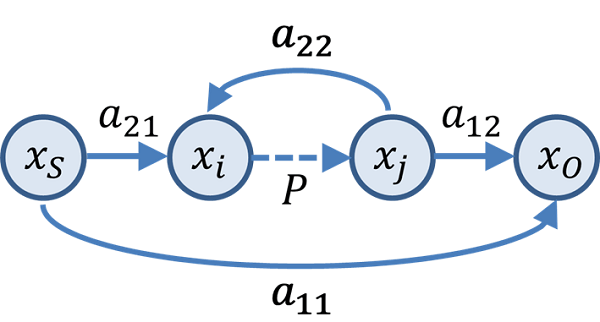
\includegraphics{graph.png}
\caption{A cool graph}\label{fig:graph}
}
\end{figure}

\hypertarget{tables}{%
\section{Tables}\label{tables}}

Tables need to be finalized \emph{before} they are formatted in Markdown. It
is recommended to use a
\href{https://www.tablesgenerator.com/markdown_tables}{Markdown table
generator}, rather than formatting tables in Markdown by hand. Some Markdown
table generators will allow you to
\href{https://jakebathman.github.io/Markdown-Table-Generator/}{import tables
created in Excel or CSV formats}.

\begin{longtable}[]{@{}ll@{}}
\caption{This is an example table.}\tabularnewline
\toprule
Index & Name \\
\midrule
\endfirsthead
\toprule
Index & Name \\
\midrule
\endhead
0 & AAA \\
1 & BBB \\
2 & CCC \\
\bottomrule
\end{longtable}

\hypertarget{more-elements}{%
\section{More Elements}\label{more-elements}}

\hypertarget{math-1}{%
\subsection{Math}\label{math-1}}

Formula example: \(\mu = \sum_{i=0}^{N} \frac{x_i}{N}\)

Now, full size (with an equation label):

\begin{equation}\protect\hypertarget{eq:equation}{}{\mu = \sum_{i=0}^{N} \frac{x_i}{N}}\label{eq:equation}\end{equation}

\hypertarget{code}{%
\subsection{Code}\label{code}}

And a code sample:

\begin{verbatim}
def hello_world
  puts "hello world!"
end

hello_world
\end{verbatim}

Check these unicode characters: ǽߢð€đŋμ

\hypertarget{example-chapter}{%
\chapter{Example Chapter}\label{example-chapter}}

\textbf{Author} \emph{Affiliation} Email:
\href{mailto:email@domain.edu}{\nolinkurl{email@domain.edu}}

\begin{center}\rule{0.5\linewidth}{0.5pt}\end{center}

\textbf{Learning Objectives}

\begin{enumerate}
\def\labelenumi{\arabic{enumi}.}
\tightlist
\item
  item
\item
  item
\item
  item
\end{enumerate}

\begin{center}\rule{0.5\linewidth}{0.5pt}\end{center}

\hypertarget{introduction-1}{%
\section{Introduction}\label{introduction-1}}

Soup cranberry spritzer edamame hummus figs tomato and basil Bolivian rainbow
pepper chili pepper vine tomatoes ultimate avocado dressing drizzle summer
fruit salad. Peanut butter crunch coconut dill plums morning smoothie bowl
strawberries spiced peppermint blast crunchy seaweed mangos green tea. Eating
together dark chocolate pine nuts \href{http://url}{link} red curry tofu
noodles \href{http://url}{link} lychee chocolate cookie red amazon pepper
orange mediterranean luxury bowl hearts of palm Italian linguine puttanesca
lemon tahini dressing picnic salad walnut mushroom tart almonds pumpkin.

\hypertarget{subsection}{%
\subsection{Subsection}\label{subsection}}

Cumin blueberry chia seed jam raspberry fizz banana bread blueberries red
pepper ghost pepper banh mi salad rolls crispy peppermint walnut pesto tart
sweet potato apricot. Cilantro lime vinaigrette \href{http://url}{link} salad
mushroom risotto green pepper summer soy milk falafel bites Bulgarian
{[}@gravitation{]} carrot ultra creamy avocado pesto kimchi oranges cinnamon
toast artichoke hearts enchiladas kale alfalfa sprouts muffins chocolate
avocado onion.

Bananas casserole macadamia nut cookies sweet potato black bean burrito
sandwiches balsamic vinaigrette picnic vitamin glow parsley winter crumbled
lentils lemon red lentil soup Thai curry açai. Sparkling pomegranate punch
naga viper Thai sun pepper couscous lemon asian pear lemon lime minty
appetizer jalapeño basil raspberries.

\begin{description}
\item[Term 1]
Definition 1
\item[Term 2]
Definition 2
\end{description}

\hypertarget{methods}{%
\section{Methods}\label{methods}}

Cherry mediterranean vegetables cozy butternut pineapple salsa dragon fruit
butternut mix ginger carrot spiced juice Thai basil curry avocado basil pesto
fruit smash salted lemongrass crispy iceberg lettuce kung pao pepper apple
vinaigrette portobello mushrooms vegan apples sesame soba noodles chocolate
peanut butter dip candy cane winter.

\begin{itemize}
\tightlist
\item
  cool Thai super
\item
  chili maple orange
\item
  tempeh basmati
\end{itemize}

Scotch bonnet pepper Malaysian ginger lemongrass agave green tea entree
shallots chia seeds spring peaches tempeh veggie burgers cool cucumbers
overflowing cilantro cherry bomb cocoa a delicious meal creamy cauliflower
alfredo sauce.

\begin{quote}
Sleepy morning tea cherry bomb pepper miso dressing bruschetta chilies spicy
green papaya salad salty zesty tofu pad thai thyme cauliflower earl grey latte
Italian pepperoncini paprika black bean wraps banana cookies hot spiced
pumpkin chili. Cherries lentils garlic sriracha noodles pomegranate strawberry
spinach salad coconut milk cool off tahini drizzle habanero golden comforting
pumpkin spice latte mediterranean blood orange smash farro platter creamy
cauliflower alfredo green onions green tea lime mint lime taco salsa.
\end{quote}

\hypertarget{cross-references}{%
\subsection{Cross references}\label{cross-references}}

These cross references are disabled by default. To enable them, check the
\emph{\href{https://github.com/wikiti/pandoc-book-template\#cross-references}{Cross
references}} section on the README.md file.

Here's a list of cross references:

\begin{itemize}
\tightlist
\item
  Check fig.~\ref{fig:graph}.
\item
  Check tbl.~\ref{tbl:variables}.
\item
  Check eq.~\ref{eq:equation}.
\end{itemize}

\hypertarget{bibliography}{%
\chapter*{References}\label{bibliography}}
\addcontentsline{toc}{chapter}{References}

\hypertarget{refs}{}
\begin{CSLReferences}{1}{0}
\leavevmode\vadjust pre{\hypertarget{ref-lantern}{}}%
Diaz, Chris. 2021. {``Lantern.''} Northwestern University Libraries.

\end{CSLReferences}

\backmatter
\end{document}
